% -*- latex -*-
%%%%%%%%%%%%%%%%%%%%%%%%%%%%%%%%%%%%%%%%%%%%%%%%%%%%%%%%%%%%%%%%
%%%%%%%%%%%%%%%%%%%%%%%%%%%%%%%%%%%%%%%%%%%%%%%%%%%%%%%%%%%%%%%%
%%%%
%%%% This text file is part of the lecture slides for
%%%% `Parallel Computing'
%%%% by Victor Eijkhout, copyright 2012-9
%%%%
%%%% Subcomm-slides.tex : slides about communicator manipulation
%%%%
%%%%%%%%%%%%%%%%%%%%%%%%%%%%%%%%%%%%%%%%%%%%%%%%%%%%%%%%%%%%%%%%
%%%%%%%%%%%%%%%%%%%%%%%%%%%%%%%%%%%%%%%%%%%%%%%%%%%%%%%%%%%%%%%%

\begin{frame}[containsverbatim]{Overview}
  In this section you will learn about various subcommunicators.

  Commands learned:
  \begin{itemize}
  \item \indexmpishow{MPI_Comm_dup}, discussion of library design
  \item \indexmpishow{MPI_Comm_split}
  \item discussion of groups
  \item discussion of inter/intra communicators.
  \end{itemize}
\end{frame}

%\sectionframe{Motivation}

\begin{frame}[containsverbatim]\frametitle{Sub-computations}
  Simultaneous groups of processes, doing different tasks, but
  loosely interacting:
  \begin{itemize}
  \item Simulation pipeline: produce input data, run simulation, post-process.
  \item Climate model: separate groups for air, ocean, land, ice.
  \item Quicksort: split data in two, run quicksort independently on the halves.
  \item Process grid: do broadcast in each column.
  \end{itemize}
  New communicators are formed recursively from \indexmpishow{MPI_COMM_WORLD}.
\end{frame}

\begin{frame}[containsverbatim]\frametitle{Communicator duplication}
Simplest new communicator: identical to a previous one.
\lstset{language=C++}
\begin{lstlisting}
int MPI_Comm_dup(MPI_Comm comm, MPI_Comm *newcomm)
\end{lstlisting}
This is useful for library writers:
\begin{lstlisting}
MPI_Isend(...); MPI_Irecv(...);
// library call
MPI_Waitall(...);  
\end{lstlisting}
\end{frame}

\frame[containsverbatim]{\frametitle{Use of a library}
  \cxxverbatimsnippet{catchmain}
}
\frame[containsverbatim]{\frametitle{Use of a library}
  \cxxverbatimsnippet{catchcalls}
}
\frame[containsverbatim]{\frametitle{Wrong way}
  \cxxverbatimsnippet{wrongcatchlib}
}

\frame[containsverbatim]{\frametitle{Right way}
  \cxxverbatimsnippet{rightcatchlib}
}

\begin{frame}[containsverbatim]\frametitle{Disjoint splitting}
  Split a communicator in multiple disjoint others.
  
Give each process a `colour', group processes by colour:
\lstset{language=C}
\begin{lstlisting}
int MPI_Comm_split(MPI_Comm comm, int color, int key, 
                   MPI_Comm *newcomm)  
\end{lstlisting}
(\n{key} determines ordering: use rank unless you want special effects)
\end{frame}

\begin{frame}[containsverbatim]\frametitle{Row/column example}
\begin{lstlisting}
MPI_Comm_rank( MPI_COMM_WORLD, &procno );
proc_i = procno % proc_column_length;
proc_j = procno / proc_column_length;

MPI_Comm column_comm;
MPI_Comm_split( MPI_COMM_WORLD, proc_j, procno, &column_comm );

MPI_Bcast( data, ... column_comm );
\end{lstlisting}
\end{frame}

\begin{frame}\frametitle{Row and column communicators}
  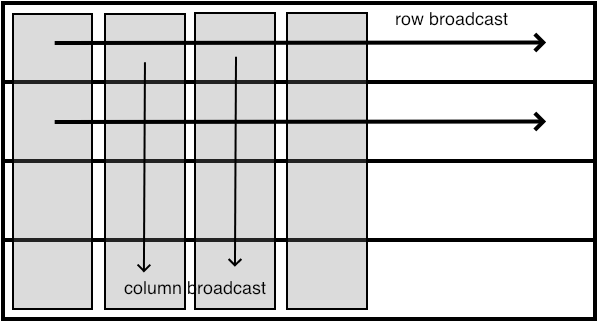
\includegraphics[scale=.1]{procgrid-bcast}

  Row and column broadcasts in subcommunicators
\end{frame}

\begin{exerciseframe}[procgrid]
  \footnotesize
  \input ex:rowcolcomm
\end{exerciseframe}

\begin{longcourse}
  \begin{exerciseframe}
    \input ex:recursivetranspose
  \end{exerciseframe}
\end{longcourse}

\begin{frame}[containsverbatim]\frametitle{Splitting by shared memory}
  \begin{itemize}
  \item
    \indexmpishow{MPI_Comm_split_type} splits into communicators of same type.
  \item Only supported type: \indexmpishow{MPI_COMM_TYPE_SHARED} splitting by
    shared memory.
  \end{itemize}

  \cverbatimsnippet{commsplittype}
\end{frame}

\begin{frame}[containsverbatim]\frametitle{More}
  \begin{itemize}
  \item Non-disjoint subcommunicators through process groups.
  \item Intra-communicators and inter-communicators.
  \item Process topologies: cartesian and graph.
  \end{itemize}
\end{frame}

\endinput

\begin{frame}[containsverbatim]\frametitle{}
\begin{lstlisting}
  
\end{lstlisting}
\end{frame}

